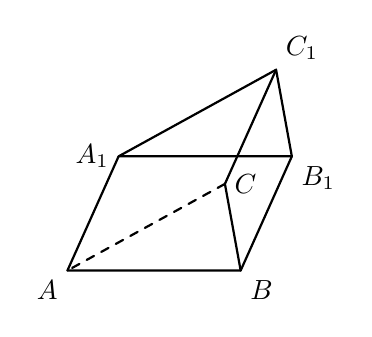
\begin{tikzpicture}[x=1cm,y=1cm,line cap=round,line join=round]
\coordinate (A) at (0,0);
\coordinate (B) at (2.2,0);
\coordinate (C) at (2.0,1.1);
\coordinate (Aone) at (0.65,1.45);
\coordinate (Bone) at (2.85,1.45);
\coordinate (Cone) at (2.65,2.55);
\draw[thick] (A)--(B)--(C);
\draw[thick,dashed] (C)--(A);
\draw[thick] (Aone)--(Bone)--(Cone)--cycle;
\draw[thick] (A)--(Aone) (B)--(Bone) (C)--(Cone);
\node[below left] at (A) {$A$};
\node[below right] at (B) {$B$};
\node[right] at (C) {$C$};
\node[left] at (Aone) {$A_1$};
\node[below right] at (Bone) {$B_1$};
\node[above right] at (Cone) {$C_1$};
\end{tikzpicture}
